\begin{question}{28}{
    Binnen Defensie wordt een phishing-oefening gedaan, waarbij naar een willekeurig geselecteerde steekproef van $300$ werknemers 
    een nep-e-mail gestuurd wordt met een verdachte link.
    Per medewerker wordt bijgehouden hoe hij/zij op de e-mail heeft gereageerd en of de medewerker een cyber-awarenesstraining heeft gevolgd.
    \par\medskip
    \begin{center}
        \renewcommand{\arraystretch}{1}
        \begin{tabular}{m{0.28\textwidth}cccc}
            \toprule
                & \textbf{Meldt e-mail} & \textbf{Negeert e-mail} & \textbf{Klikt op link} & \textbf{Totaal} \\
            \midrule
                \textbf{Cybertraining} & $72$ & $55$ & $30$ & $157$  \\
                \textbf{Geen cybertraining} & $62$ & $37$ & $44$ & $143$ \\
            \midrule
                \textbf{Totaal} & $134$ & $92$ & $74$ & $300$ \\
            \bottomrule
        \end{tabular}
    \end{center}
    De Defensiestaf wil graag weten of het gevolgd hebben van cyber-awarenesstraining daadwerkelijk invloed heeft gehad op het adequaat reageren op de nep-e-mail.
}

    \subquestion{3}{
        Wat voor type hypothesetoets zou geschikt zijn om dit te kunnen toetsen?
        Formuleer de bijbehorende nulhypothese $H_0$ en de alternatieve hypothese $H_1$ voor deze toets.
    }

    \solution{
        Om te bepalen of er een statistisch significant effect is van het al dan niet volgen van de cyber-awarenesstraining voor het adequaat reageren
        op een nep-e-mail, dienen we een chikwadraattoets voor onafhankelijkheid uit te voeren. \rubric{1}
        De nulhypothese $H_0$ en de alternatieve hypothesetoets $H_1$ kunnen dan als volgt worden geformuleerd:
        \begin{itemize}
            \item[$H_0$:] er is sprake van onafhankelijkheid tussen het wel/niet volgen van de training en het type reactie op de nep-e-mail.\rubric{1}
            \item[$H_1$:] er is GEEN sprake van onafhankelijkheid tussen het wel/niet volgen van de training en het type reactie op de nep-e-mail. \rubric{1}
        \end{itemize}
    }

    \subquestion{8}{
        Wat is de theoretische toetsingsgrootheid van deze hypothesetoets?
        Bereken de geobserveerde toetsingsgrootheid met behulp van de data in bovenstaande tabel.
    }
    \solution{
        De (theoretische) toetsingsgrootheid voor een chikwadraattoets voor onafhankelijkheid is gelijk aan
        \[
            X^2 = \sum_{i,j} \frac{(O_{ij}-E_{ij})^2}{E_{ij}}.\rubric{1}
        \]    
        Voordat we de toetsingsgrootheid kunnen berekenen, moeten we dus de verwachte frequenties $E_{ij}$ bepalen.
        Dit doen we aan de hand van de volgende formule:
        \[
            E_{ij} = \frac{(\text{rijtotaal}_i) \cdot (\text{kolomtotaal}_j)}{\text{totaal}} \rubric{1}
        \]
        We berekenen de verwachte frequenties voor elke cel in de tabel:
        \par\medskip
        \begin{center}
            \renewcommand{\arraystretch}{1}
            \begin{tabular}{m{0.28\textwidth}|ccc|c}
                \toprule
                    & \textbf{Meldt e-mail} & \textbf{Negeert e-mail} & \textbf{Klikt op link} & \textbf{Totaal} \\
                \midrule
                \textbf{Cybertraining} & $70.1267$ & $48.1467$ & $38.7267$ & $157$ \\ 
            \textbf{Geen cybertraining} & $63.8733$ & $43.8533$ & $35.2733$ & $143$ \\ 
                \midrule
                    \textbf{Totaal} & $134$ & $92$ & $74$ & $300$ \rubric{3} \\
                \bottomrule
            \end{tabular}
        \end{center}
        \par\medskip
        Vervolgens berekenen we de geobserveerde toetsingsgrootheid $\chi^2$ als volgt:
        \begin{align*}
            \chi^2 &= \frac{(o_{1, 1} - e_{1,1})^2}{e_{1, 1}} + \frac{(o_{1, 2} - e_{1,2})^2}{e_{1, 2}} + \ldots + \frac{(o_{2, 3} - e_{2,3})^2}{e_{2, 3}} \\
                    &= \frac{(72 - 70.1267)^2}{70.1267} + \frac{(55 - 48.1467)^2}{48.1467} + \ldots + \frac{(44 - 35.2733)^2}{35.2733} \\
                    &\approx 6.2770. \rubric{3}
        \end{align*}
    }

    \subquestion{5}{
        Wat is de kansverdeling van de theoretische toetsingsgrootheid onder $H_0$? 
        Bereken met deze kansverdeling de $p$-waarde behorende bij de geobserveerde toetsingsgrootheid.
    }
    \solution{
        De theoretische toetsingsgrootheid $X^2$ volgt onder de nulhypothese een chikwadraatverdeling met $\df = (\#\text{rijen}-1)\cdot(\#\text{kolommen}-1) = (2-1)\cdot(3-1) = 2$ vrijheidsgraden. \rubric{2}
        De $p$-waarde is de kans dat de theoretische toetsingsgrootheid $X^2$ een \enquote{nog extremere} uitkomst aanneemt dan de geobserveerde toetsingsgrootheid $\chi^2$. \rubric{1}
        
        Aangezien een chikwadraattoets voor onafhankelijkheid altijd rechtszijdig is, is de $p$-waarde gelijk aan
        \begin{align*}
            p   &= P(\chi^2 > 6.2770) \\ 
                &= \chi^2\text{cdf}(\lb=6.2770; \ub=10^{99}, \df=2) \\
                &\approx 0.0433.  \rubric{2} 
        \end{align*}

        \begin{center}
            \resizebox{0.9\textwidth}{!}{
                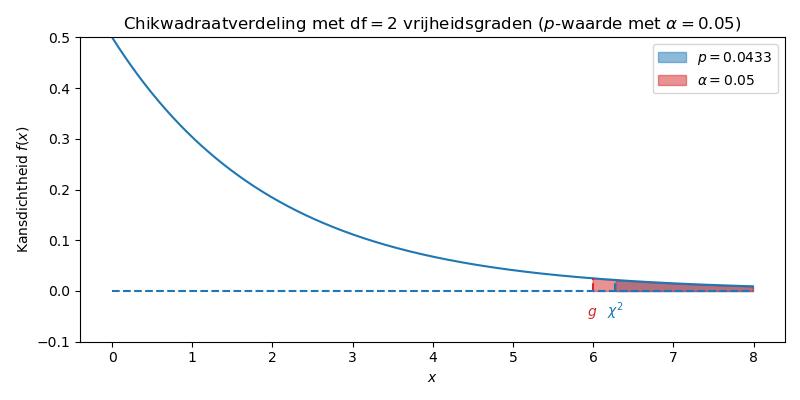
\includegraphics{exam20261106-chi2-pvalue.png} 
            }
        \end{center}
    }

    \subquestion{4}{
        Bepaal de toetsuitslag op basis van de berekende $p$-waarde en vertaal deze terug naar de originele probleemcontext.
        Gebruik hiervoor een significantieniveau $\alpha = 0.05$.
        Geef een verklaring voor de toetsuitslag met behulp van de tabel van geobserveerde en verwachte frequenties.
    }
    \solution{
        Aangezien de $p$-waarde $p \approx 0.0433$ strikt kleiner is dan het significantieniveau $\alpha = 0.05$,
        besluiten we om de nulhypothese $H_0$ te verwerpen. \rubric{1}

        Er is voldoende reden om aan te nemen dat het gevolgd hebben van een cyber-awarenesstraining
        significant effect heeft op de manier waarop op een nep-e-mail wordt gereageerd. \rubric{1}
        
        Als we kijken naar de tabellen van geobserveerde en verwachte frequenties,
        dan zien we dat voor de cellen met kenmerk \enquote{klikt op e-mail} de groep die geen training gevolgd heeft vaker dan verwacht (onder onafhankelijkheid) op de link heeft geklikt,
        terwijl dit bij de groep die wel training gevolgd heeft andersom is.\rubric{2}
    }
    
    \subquestion{8}{
        De commandant van de cybereenheid die deze nep-e-mail heeft verspreid beweert dat \SI{20}{\percent} van de Defensiemedewerkers op de link klikt.
        Bereken met de Clopper-Pearson methode een \SI{95}{\percent}-betrouwbaarheidsinterval voor de kans $p$ dat een willekeurige medewerker op de link klikt.
        Wat kunnen we concluderen over de claim van de commandant?
    }

    \solution{
        Van de $300$ medewerkers naar wie de link is verstuurd, hebben $30+44 = 74$ medewerkers op de link gedrukt (steekproef!).\rubric{1}
        Ervan uitgaande dat iedere medewerker onafhankelijk van elkaar wel of niet op de klik drukt, is het aantal medewerkers dat op
        de link drukt een binomiale kansvariabele $X$ met $n = 300$ en een onbekende succeskans $p = \text{ ?}$. \rubric{1}
        Op basis van deze aantallen gaan we een betrouwbaarheidsinterval bepalen voor de kans $p$ dat een willekeurige medewerker
        op de link drukt (populatieparameter!).
        Omdat de gewenste betrouwbaarheid \SI{95}{\percent} is, geldt dat $\alpha = 0.05$.

        De Clopper-Pearson methode werkt als volgt:
        \begin{enumerate}
            \item Bepaal de minimale succeskans $p_1$ waarvoor de uitkomst $k = 74$ niet extreem groot is, oftewel $P(X \geq 74) = 1 - P(X \leq 73) = \alpha/2 \geq 0.025$.
            Voer hiervoor in de \enquote{numerieke solver} van de grafische rekenmachine in:
            \begin{align*}
                E_1 &= 1 - \binomcdf(n=300, p_1=X, k=74) \\
                E_2 &= 0.025 
            \end{align*}
            De \enquote{numerieke solver} geeft een waarde van $p_1 \approx 0.1989$.
            \item Bepaal de maximale succeskans $p_2$ waarvoor de uitkomst $k = 74$ niet extreem klein is, oftewel $P(X \leq 74) = \alpha/2 \geq 0.025$.
            Voer hiervoor in de \enquote{numerieke solver} van de grafische rekenmachine in:
            \begin{align*}
                E_1 &= \binomcdf(n=300, p_1=X, k=74) \\
                E_2 &= 0.025 
            \end{align*}
            De \enquote{numerieke solver} geeft een waarde van $p_2 \approx 0.2995$.
        \end{enumerate}
        We vinden het Clopper-Pearson interval door de twee gevonden waarden als grenzen te nemen,
        oftewel het \SI{95}{\percent}-betrouwbaarheidsinterval voor de kans $p$ dat een willekeurige medewerker op de link klikt
        is gelijk aan $[0.1989, 0.2995]$. \rubric{4}

        We zien dat de geclaimde succeskans $p = 0.20$ in het Clopper-Pearson interval ligt. \rubric{1}
        Deze geobserveerde steekproefresultaten geven dus onvoldoende reden om de claim van de commandant naast ons neer te leggen.\rubric{1}
    }
\end{question}